\section*{Exercice 143 -- Fonctions de transfert}
\setcounter{exo}{0}
%CCS PSI 2005


\begin{obj}
Vérifier les performances de l’asservissement d’inclinaison par rapport à la verticale.
\end{obj}

Pour une utilisation confortable et sûre, le Segway doit satisfaire les performances
énoncées dans le tableau extrait du cahier des charges.
\begin{center}
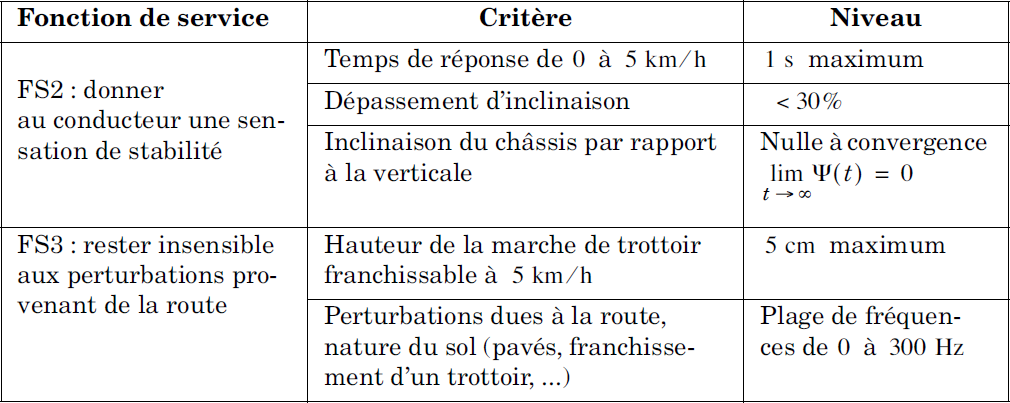
\includegraphics[width=\linewidth]{976_01}%
\end{center}
La régulation d’inclinaison du Segway® est réalisée par :
\begin{itemize}
\item un moto-réducteur qui permet de délivrer un couple $C_m(t)=K_m u(t)$ où $u(t)$ est une grandeur de commande et $K_m=\SI{24}{N.m.V^{-1}}$;
\item le système mécanique dont les équations, dans le cas où l’angle $\alpha(t)$ n’est pas supposé constant, se met
sous la forme :
$\left\{
\begin{array}{l}
\dot{V}(t)=\dfrac{1}{D}\left( B\ddot{\chi}(t)+2\dfrac{C_m(t)}{R}\right) \\
\left(DA-B^2\right)\ddot{\chi}(t)=2\left(\dfrac{B}{R}+D\right)C_m(t)+DC\chi(t)
\end{array}
\right.
$ 
avec
$\left\{
\begin{array}{l}
A=\SI{90}{kg.m^2} \\
B=\SI{75}{kg.m} \\
C=\SI{750}{kg.m^2.s^{-2}} \\
D=\SI{125}{kg} \\
R=\SI{240}{mm} \\
\chi(t)=\alpha(t)+\psi(t) 
\end{array}
\right.
$.
\end{itemize}


Par commodité de signe, la notation est utilisée dans les équations ci-dessus. Les conditions initiales sont toutes nulles.


\subparagraph{}
\textit{Montrer que le schéma bloc du système peut se mettre sous la forme suivante en déterminant l’expression littérale de $H_1(p)$.}
\ifprof
\begin{corrige}
\end{corrige}
\else
\fi

\begin{center}
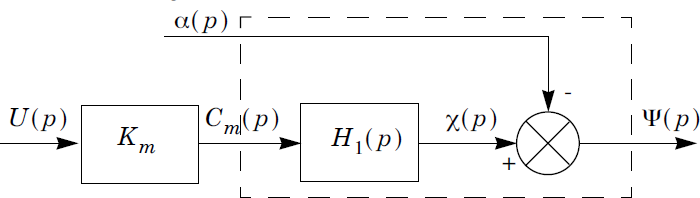
\includegraphics[width=\linewidth]{976_02}%
\end{center}


\subparagraph{}
\textit{Analyser la stabilité du système d’entrée $u(t)$ et de sortie $\psi(t)$ en étudiant la fonction de transfert $F_1(p)=\dfrac{\Psi(p)}{U(p)}$.}% Pouvait-on s'attendre à ce résultat ?}
\ifprof
\begin{corrige}
\end{corrige}
\else
\fi


On note alors $H_1(p)=\dfrac{K_1}{\dfrac{p^2}{\omega_1^2} - 1}$. 

Les valeurs numériques utilisées par la suite seront : $\omega_1=\SI{4,1}{rad.s^{-1}}$ et
$K_S = K_mK_1 = \SI{0,24}{rad.V^{-1}}$.

Afin de stabiliser le système, la grandeur de commande $U(p)$ est élaborée à partir des mesures de $\dot{\Psi}$ (réalisée par le gyromètre), et de ${\Psi}$( (réalisée par combinaison de la mesure du gyromètre et du pendule). Le schéma-blocs obtenu est celui du document réponse.


\subparagraph{}
\textit{Dans le cas où $\alpha = 0$, déterminer, en fonction de $K_S$, $k_p$, $k_v$ et $\omega_1$ la
fonction de transfert $F_2(p)=\dfrac{\Psi(p)}{W(p)}$.}
\ifprof
\begin{corrige}
\end{corrige}
\else
\fi



\subparagraph{}
\textit{Déterminer les conditions sur $k_v$ et sur $k_p$ pour que le système soit stable.}
\ifprof
\begin{corrige}
\end{corrige}
\else
\fi

$F_2(p)$ est une fonction de transfert du second ordre pouvant se mettre sous la forme :
$F_2(p)=\dfrac{\Psi(p)}{W(p)}=\dfrac{K_2}{1+\dfrac{2\xi}{\omega_0}p+\dfrac{p^2}{\omega_0^2}}$.


\subparagraph{}
\textit{Déterminer les expressions de $K_2$, $\xi$ et $\omega_0$.}
\ifprof
\begin{corrige}
\end{corrige}
\else
\fi

On choisit une pulsation propre proche de celle du système mécanique, c’est
à dire $\omega_0 = 1,5\omega_1=\SI{6,15}{rad.s^{-1}}$.



\subparagraph{}
\textit{Déterminer les valeurs de $k_p$ et de $k_v$ telles que le temps de réponse à 5\% soit minimal.}
\ifprof
\begin{corrige}
\end{corrige}
\else
\fi



%\subparagraph{}
%\textit{}
%\ifprof
%\begin{corrige}
%\end{corrige}
%\else
%\fi


\begin{enumerate}
\item ...
\item ...
\item $F_2(p)=\dfrac{K_S}{\dfrac{p^2}{\omega_1^2}+pk_v K_S +k_pK_S - 1}$.
\item $k_p>\dfrac{1}{K_S}$ et $k_v>0$.
\item $K_2 = \dfrac{K_S}{k_p K_S - 1}$, $\omega_0 = \omega_1\sqrt{k_p K_S - 1}$ et $\xi = \dfrac{1}{2}\dfrac{k_vK_S\omega_1}{\sqrt{k_p K_S - 1}}$.
\item $k_v = \SI{2,15}{rad.s^{-1}s}$, $K_2 \simeq \SI{0,1}{rad.V^{-1}}$, $k_p \simeq \SI{13,54}{V.rad^{-1}}$.
\end{enumerate}